\section{Оптимизация направленности ФАР: основные понятия, постановка задач, проблемы и методы решения}
\subsection{Основные понятия}
\begin{frame}[plain, noframenumbering]
    \begin{center}
        \Huge
        Оптимизация направленности ФАР: основные понятия, постановка задач, проблемы и методы решения
    \end{center}
\end{frame}

\begin{frame}[plain, noframenumbering]
    \frametitle{Основные понятия}
    \begin{center}
        \begin{figure}
            \begin{minipage}[h]{0.42\linewidth}
                \center{\includegraphics[width=1\linewidth]{2x2bve.eps} \\ а)}
            \end{minipage}
            \hfill
            \begin{minipage}[h]{0.42\linewidth}
                \center{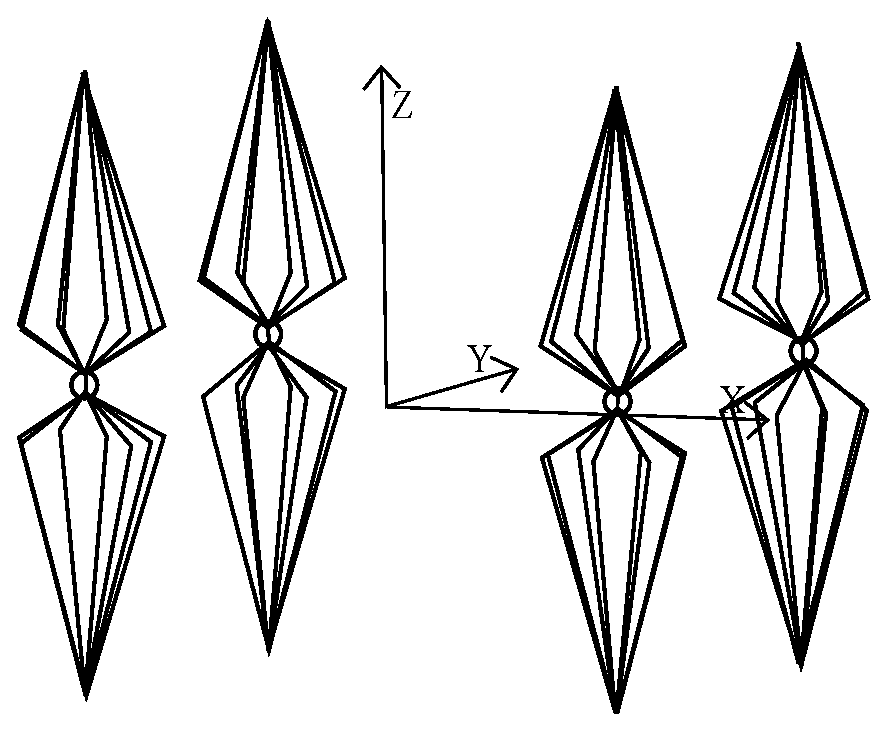
\includegraphics[width=0.6\linewidth]{2x2bvd.eps} \\ б)}
            \end{minipage}
            \begin{minipage}[h]{0.42\linewidth}
                \center{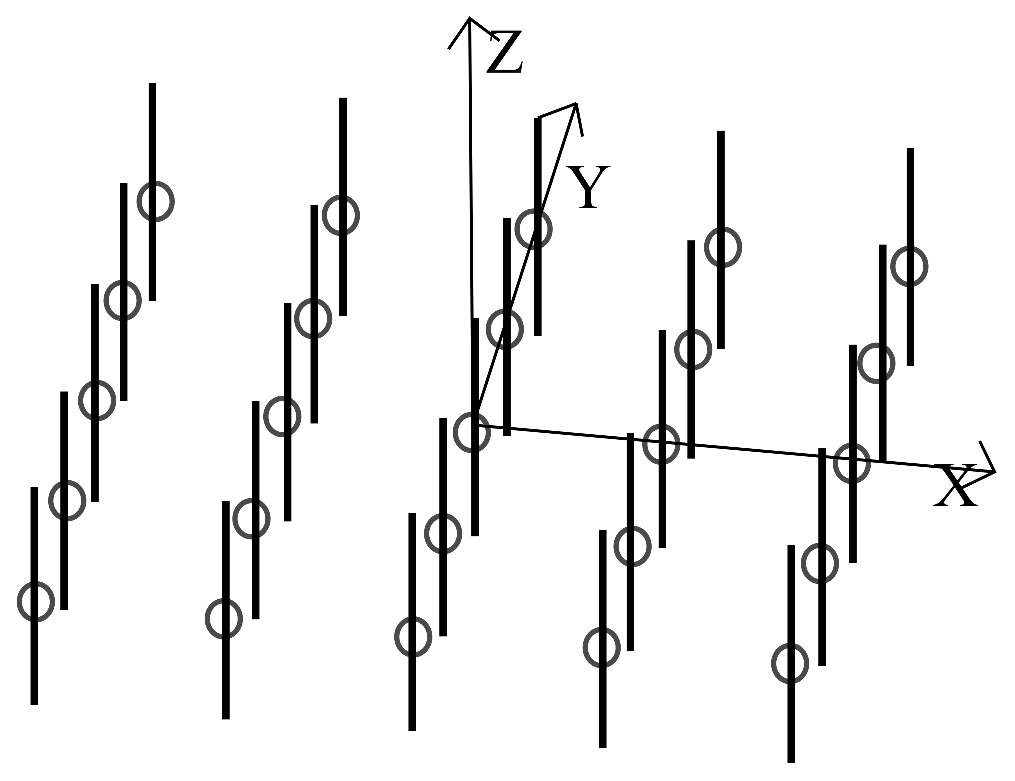
\includegraphics[width=0.6\linewidth]{5x5VWD.eps} \\ в)}
            \end{minipage}
            \hfill
            \begin{minipage}[h]{0.42\linewidth}
                \center{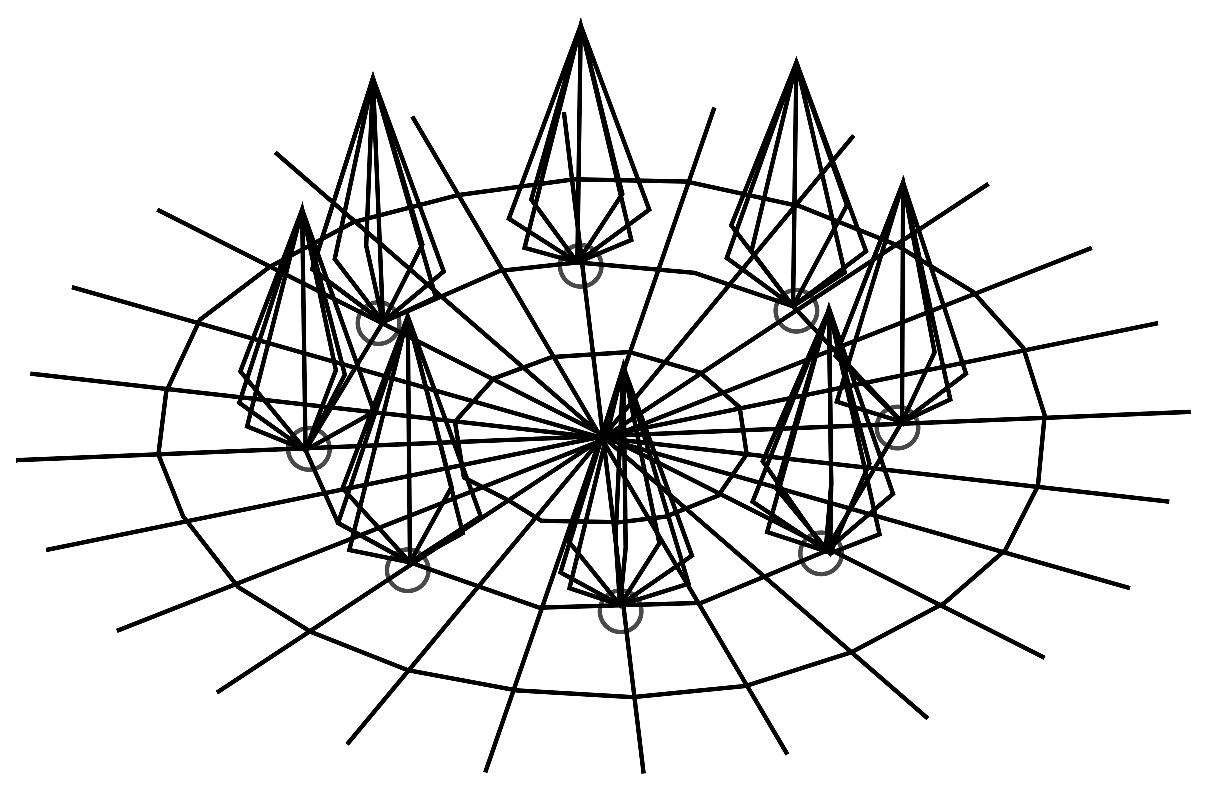
\includegraphics[width=0.9\linewidth]{r8.eps} \\ г)}
            \end{minipage}
            \label{ris:bve_bvd}
            \caption{ФАР различных конфигураций}
        \end{figure}

    \end{center}
    \footnotesize { \textbf{Юрков А.С.:} Оптимизация возбуждения передающих фазированных антенных решеток декаметрового диапазона длин волн. ОНИИП, Омск (2014)\\
    \textbf{Fuchs B.:} Application of convex relaxation to array synthesis problems. IEEE, P.~634-640, 2014.
    }
\end{frame}

\begin{frame}
    \frametitle{Положения, выносимые на защиту}
    \begin{itemize}
        \item В задаче имеется одномерная непрерывная группа симметрий.
        \item Имеются конфигурации ФАР, при которых учет взаимного влияния излучателей ведет к существенному увеличению коэффициента усиления в заданном направлении.
        \item Для многих конфигураций ФАР задача имеет несколько кластеров из локальных оптимумов с одинаковым значением целевой функции, не эквивалентных относительно равного сдвига фаз во всех излучателях.
    \end{itemize}
\end{frame}
\note{
    Проговариваются вслух положения, выносимые на защиту
}

\subsection{Постановка задачи}
\begin{frame}
    \frametitle{Постановка в комплексных числах}
    \begin{equation}
    f^{(l)}_{\Sigma} = \sum_{i=1}^{N}I_i \tilde{f}_i^{(l)}
    \label{eq:sumfield}
    \end{equation}

     \begin{equation}
        F = \sum_{l=1}^{2}\overline{f}_{\Sigma}^{(l)}f_{\Sigma}^{(l)}
        \label{eq:FPrimary}
    \end{equation}
    
        \begin{equation}
        F = \textbf{i}^{+}\textbf{Ai} \rightarrow \max
        \label{eq:F}
    \end{equation}

\vspace{2em}
    \textbf{Юрков А.С.:} Оптимизация возбуждения передающих фазированных антенных решеток декаметрового диапазона длин волн~// ОНИИП 2014. 
\end{frame}

\begin{frame}
    \frametitle{Постановка в комплексных числах}
   \begin{equation}
        \begin{cases}
           \textbf{i}^{+}\textbf{Ai} \rightarrow \max,\\
           0 \leq \textbf{i}^{+}\textbf{B}^{(1)}\textbf{i} \leq 1, \\
           ...\\
           0 \leq \textbf{i}^{+}\textbf{B}^{(n)}\textbf{i} \leq 1,\\
           \textbf{i} \in \mathbb{C}^N\\
         \end{cases}
         \label{eq:task2}
    \end{equation}
%
где $n$ - число точек питания, на которые накладываются ограничения
%
    \begin{equation}
        \textbf{B}^{(k)} = \frac{1}{4P_{max}^{(k)}}(\textbf{Z}^{+}\mathcal{P}^{(k)} + \mathcal{P}^{(k)}\textbf{Z}) \, ,
    \end{equation}
%
$P_{max}^{(k)}$ - максимально допустимая мощность в $k$-й точке питания, $\mathcal{P}^{(k)}$ - матрицы-проекторы имеющие единственный ненулевой элемент $\mathcal{P}^{(k)}_{kk}=1$.

\vspace{2em}
    \textbf{Юрков А.С.:} Оптимизация возбуждения передающих фазированных антенных решеток декаметрового диапазона длин волн~// ОНИИП 2014.
\end{frame}

\begin{frame}
    \frametitle{Постановка в комплексных числах}
   \begin{enumerate}
  \item Все матрицы $\textbf{B}^{(k)}$ имеют не больше чем два ненулевых собственных значения. Одно из собственных значений положительно,
  остальные отрицательные или нулевые.
  \item Матрицы $\textbf{A}$ и $\textbf{B}^{(k)}$ эрмитово-самосопряженные, то есть
  $a_{ij} = \overline{a}_{ji}$ для всех $i = \overline{1,N}, j = \overline{1,N}$.
  \item Матрица $\textbf{A}$ положительно полуопределена.
  \item Кроме того, из физических соображений вытекает, что матрица $\textbf{B}_{\Sigma}:= \sum_{k=1}^{n} \textbf{B}^{(k)}$
  положительно определена, так как суммарная активная мощность, поглощаемая пассивной цепью, не может быть отрицательной либо нулем,
  поскольку, часть энергии обязательно излучится.
\end{enumerate}

\vspace{2em}
    \textbf{Юрков А.С.:} Оптимизация возбуждения передающих фазированных антенных решеток декаметрового диапазона длин волн~// ОНИИП 2014.
\end{frame}

\begin{frame}
    \frametitle{Постановка в вещественных числах}
    \begin{equation}
        \begin{cases}
           \textbf{x}^{T}\textbf{Gx} \rightarrow \max,\\
           0 \leq \textbf{x}^{T}\textbf{H}^{(1)}\textbf{x} \leq 1,\\
           ...\\
           0 \leq \textbf{x}^{T}\textbf{H}^{(n)}\textbf{x} \leq 1,\\
          \textbf{x} \in \mathbb{R}^{2n}.\\
         \end{cases}
         \label{eq:task3}
    \end{equation}
Задача~(\ref{eq:task3}) имеет целевую функцию, заданную квадратичной формой с положительно полуопределенной матрицей~$\textbf{G}$. Каждое ограничение формулируется квадратичной формой, определенной симметричной матрицей~$\textbf{H}^{(k)}, k=\overline{1,n}$ с двумя парами идентичных собственных значений, два из которых положительны, а другие два отрицательны или равны нулю, все остальные собственные числа равны нулю.

\vspace{2em}


\footnotesize { \textbf{Ereemeev A.V., Tynin N.N., Yurkov A.S.:} Non-Convex Quadratic Programming Problems in Short Wave Antenna Array Optimization.~// MOTOR 2019 (11584) }
\end{frame}


\begin{frame}
    \frametitle{Верхняя оценка нормы допустимых решений}
    
    Если $\bf x$ удовлетворяет всем ограничениям задачи~(\ref{eq:task3}), то
$$
\sum_{k=1}^{n} {\bf x}^T {\bf H}^{(k)}  {\bf x} \le N.
$$
$${\bf H}_{\rm sum}:= \sum_{k=1}^{n} {\bf H}^{(k)}$$
$$\lambda_{\min} > 0$$
$$
\min\{{\bf z}^T {\bf H}_{\rm sum} {\bf z} \ : \ {\bf z}\in
\mathbb{R}^{2N}, \ ||{\bf z}|| =1\} = \lambda_{\min},
$$
$$
{\bf x}^T {\bf H}_{\rm sum} {\bf x} \ge ||{\bf x}||^2
\lambda_{\min}\ \
$$
\begin{equation} \label{eqn:bound}
||{\bf x}||\le \sqrt{\frac{N}{\lambda_{\min}}}.
\end{equation}

\vspace{2em}

\footnotesize { \textbf{Тюнин Н.Н.:} Задачи невыпуклого квадратичного программирования, связанные с оптимизацией фазированных антенных решеток~//Дискретный анализ и исследование операций, 2021, 28(3)}

\end{frame}


\begin{frame}
    \frametitle{Масштабирование решения в допустимую область}

Если решение $\textbf{x}$ нарушает только ограничивающие неравенства задачи~(\ref{eq:task3}) вида $\textbf{x}^{T}\textbf{H}^{(k)}\textbf{x} \leq 1,$ то:

\begin{equation}
    {\bf x}': =\mu({\bf x})^{-1/2} {\bf x} ,
    \label{eq:scale}
\end{equation}
где $\mu({\bf x}):=\max_{k=\overline{1,n}} {\bf x}^T {\bf H}^{(k)}{\bf x}$.
\vspace{2em}

\footnotesize { \textbf{Тюнин Н.Н.:} Задачи невыпуклого квадратичного программирования, связанные с оптимизацией фазированных антенных решеток~//Дискретный анализ и исследование операций, 2021, 28(3)}

\end{frame}

\begin{frame}
    \frametitle{Постановка задачи}
    \begin{block}{Метод штрафных функций}
        \begin{equation}
               \textbf{x}^{T}\textbf{Gx} - r\cdot \sum_{k=1}^n
               \left( \min\left(0,\textbf{x}^{T}\textbf{H}^{(k)}\textbf{x}\right) +
               \min\left(0,1-\textbf{x}^{T}\textbf{H}^{(k)}\textbf{x}\right)\right)^{\alpha} \rightarrow
               \max
             \label{eq:task4}
        \end{equation}
    \end{block}

    \begin{block}{Необходимые условия локальной оптимальности}
        \begin{equation}
            \begin{cases}
               \textbf{x}_0^T\textbf{G}\textbf{x}_0 + 2\textbf{x}_0^T\textbf{G}\textbf{y} \rightarrow \max,\\
               0 \leq \textbf{x}_0^T\textbf{H}^{(1)}\textbf{x}_0 + 2\textbf{x}_0^T\textbf{H}^{(1)}\textbf{y} \leq 1,\\
               ...\\
               0 \leq \textbf{x}_0^T\textbf{H}^{(n)}\textbf{x}_0 + 2\textbf{x}_0^T\textbf{H}^{(n)}\textbf{y} \leq 1,\\
              \textbf{y} \in \mathbb{R}^{2N}.\\
             \end{cases}
             \label{eq:task5}
        \end{equation}
    \end{block}
\end{frame}

%------------------------------------------------
\subsection{Вычислительный эксперимент}
\begin{frame}
    \frametitle{ Вычислительный эксперимент }
    Цели эксперимента
    \begin{itemize}
      \item Исследование структуры локальных оптимумов
      \item Сравнение эффективности работы различных алгоритмов
      \item Исследование возможностей ФАР в разных условиях
    \end{itemize}
    Исследуемые алгоритмы
    \begin{itemize}
      \item Градиентный подъем 
      \begin{itemize}
        \item Выбор начального значения в пределах оцененной нормы
        \item Масштабирование решения в допустимую область
      \end{itemize}
      \item BARON
    \end{itemize}
    Детали эксперимента
    \begin{itemize}
      \item Антенный моделировщик NEC2
      \item Направление оптимизации $70^{\circ}:45^{\circ}$
    \end{itemize}
\end{frame}

\begin{frame}
    \frametitle{ Программный комплекс}

    \begin{figure}
    \centering
        \begin{minipage}[h]{1\linewidth}
                \center{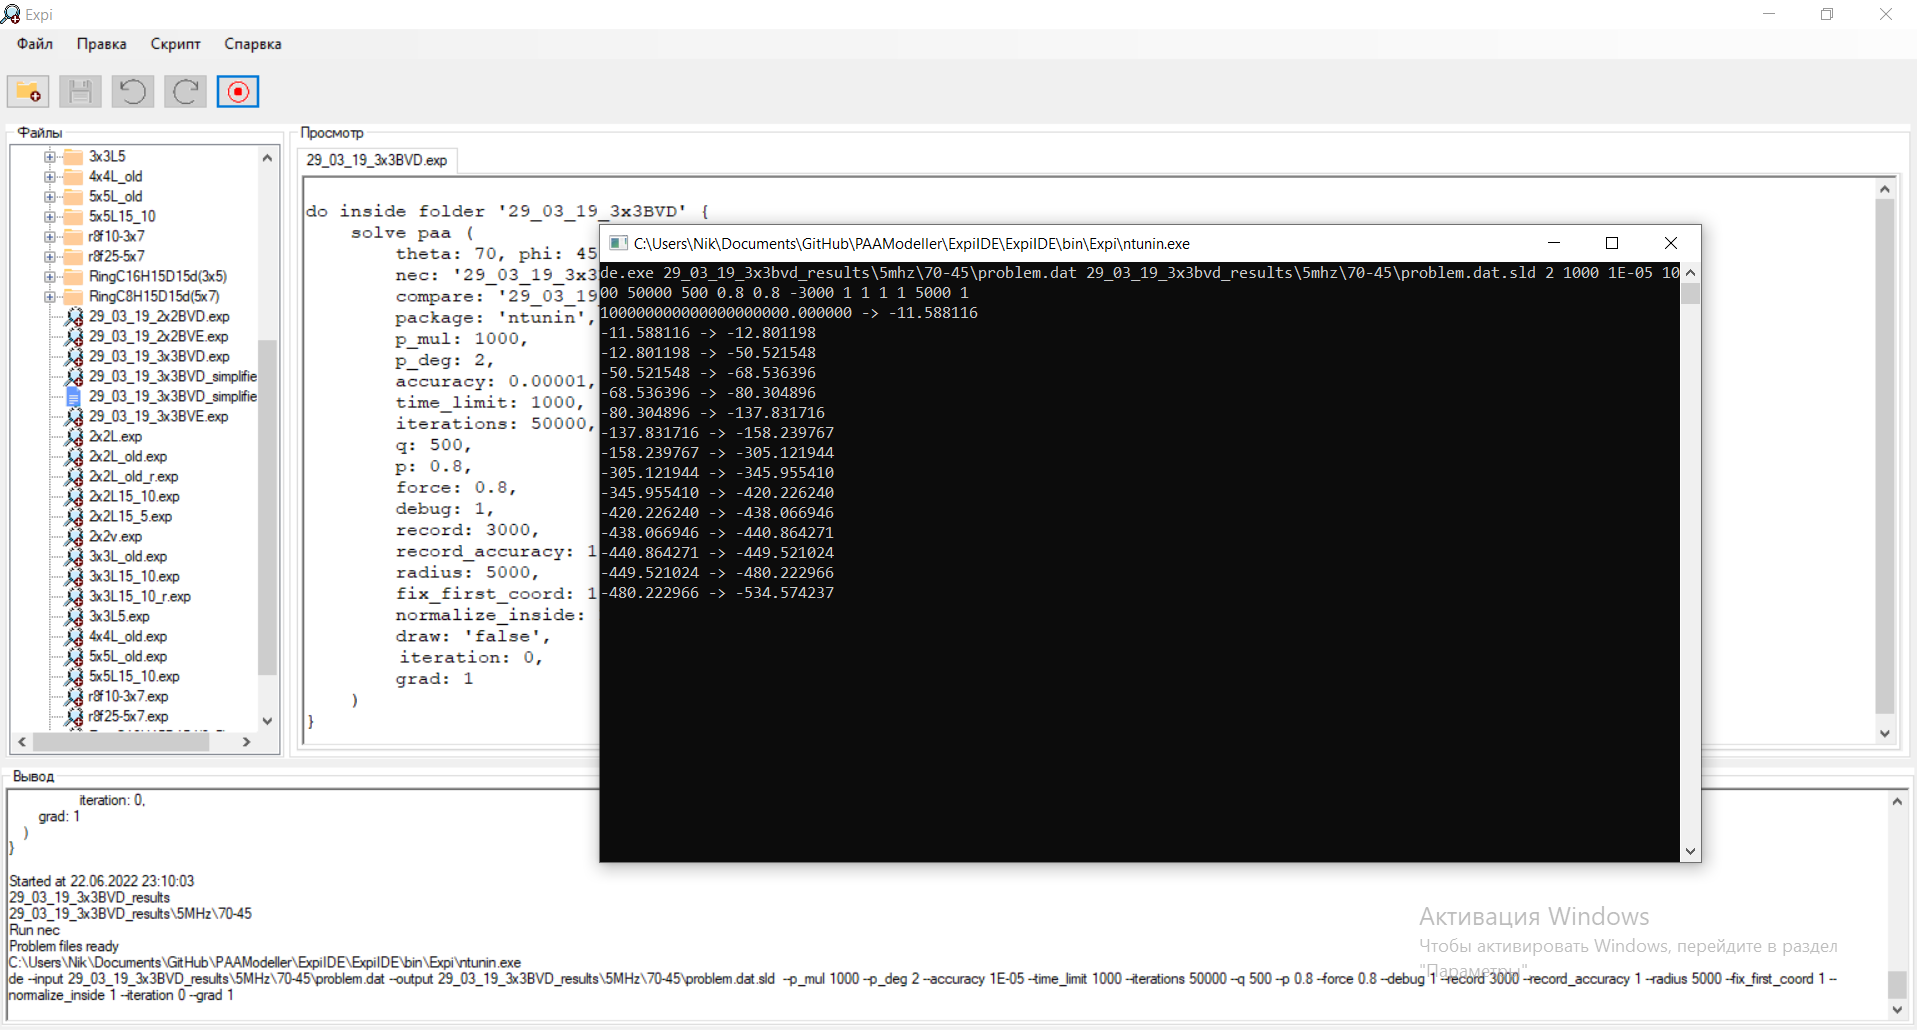
\includegraphics[width=0.9\linewidth]{expi.png} }
        \end{minipage}
        \vspace{0.7em}
        \caption{Графический интерфейс программного комплекса}
        \label{ris:expi}
    \end{figure}

\end{frame}

\begin{frame}
    \frametitle{Сравнение результатов оптимизации градиентного подъема и решателя BARON}
    \begin{table}
\centering
\begin{tabular}{|c|c|c|c c|c c|}
    \hline
    \multirow{2}{*}{\textbf{ФАР}} & \multirow{2}{*}{$\lambda_{min}$} & \multirow{2}{*}{$\sqrt{\frac{N}{\lambda_{\min}}}$} & \multicolumn{2}{c}{\textbf{Град.}} & \multicolumn{2}{|c|}{\textbf{BARON}}\\
    & & & \textbf{$\textbf{F}$} & \textbf{t, c} & \textbf{$\textbf{F}$} & \textbf{t, c} \\
    \hline
    ШВИ 2х2 & 0.0215 & 13.6 & 138.2 & \textbf{0.054} & \textbf{139.2} & 0.12 \\
    ШВИ 3х3 & 0.0177 & 70 & 575.7 & 0.93 & \textbf{580.6} & \textbf{0.34} \\
    ШВД 2х2 & 0.009 & 21 & 459.7 & \textbf{0.13} & \textbf{463.6} & 0.27 \\
    ШВД 3х3 & 0.0013 & 6767 & 915 & 24.4 & \textbf{925} & \textbf{0.34}  \\
    СВД 2х2 & $2\cdot10^{-3}$ & 44& 357 & 1.9 & \textbf{361} & \textbf{0.16} \\
    СВД' 3х3 & 0.0008 & $1\cdot10^4$& 664 & 71 & \textbf{1153} & \textbf{1.48} \\
    СВД' 5х5 & - & - & \textbf{1382.7} & 1000 & 33.5 & \textbf{217.94}  \\
    Кольц. 8 & $3\cdot10^{-3}$ & 154 & 217 & 8.06 & \textbf{218} & \textbf{0.23} \\
    Кольц. 16 & $6.7\cdot10^{-4}$ & $1.2\cdot10^{6}$& 727 & 90.9 & \textbf{734} & \textbf{1.37} \\
    \hline
\end{tabular}
\label{tab:results}
\end{table}

$\sqrt{\frac{N}{\lambda_{\min}}}$ - оценка сверху евклидовой нормы.
\end{frame}


%------------------------------------------------
\begin{frame}
    \frametitle{Экспериментальная проверка устойчивости решений}
    \begin{figure}[h]
    \centering
    \center{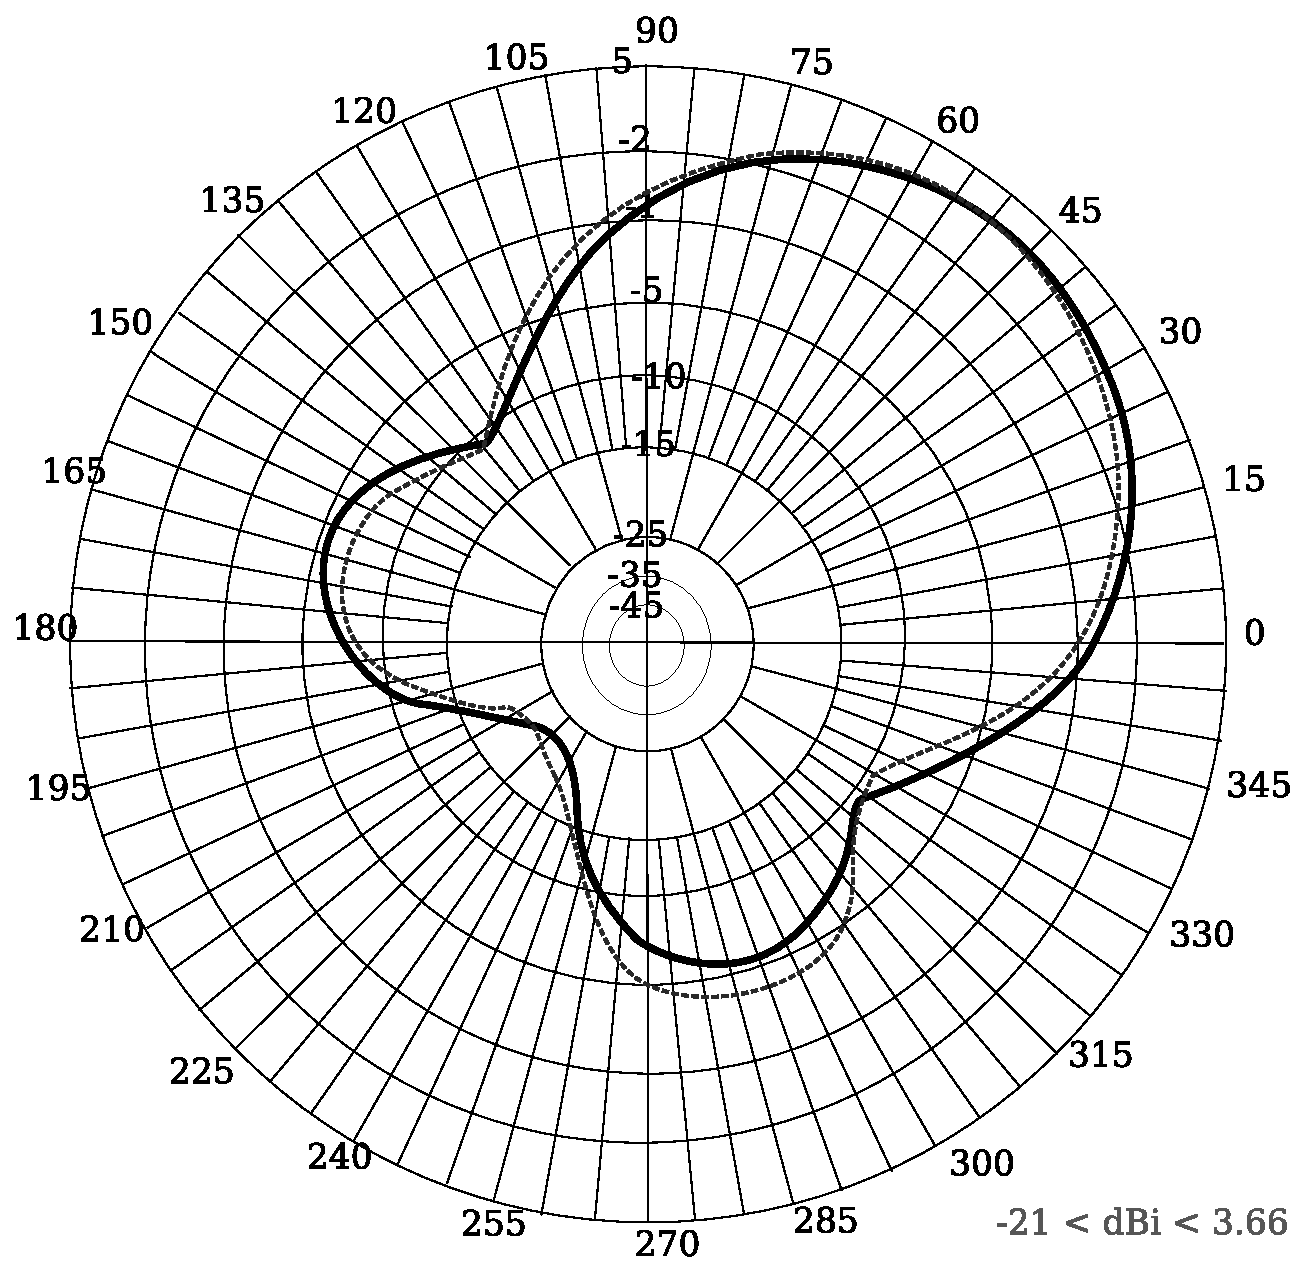
\includegraphics[width=0.5\linewidth]{stability.eps} }
    \vspace{0.7em}
    \caption{Диаграммы направленности для ШВИ~2x2 при оптимизации в направлении 70:45 (сплошная линия) и 70:50 (пунктир)}
    \label{ris:bve_comp}
    \end{figure}
\end{frame}

\subsection{Группы симметрий}


\begin{frame}
    \frametitle{Группы симметрий}
  Под линейной симметрией задачи будем понимать линейное преобразование P пространства поиска, имеющее вид~(\ref{eq:linsim}), заданное невырожденной матрицей $\textbf{P}$, такое что при подстановке новых координат y задача совпадает с исходной.% (т. е. все квадратичные формы от y оказываются теми же, что и исходные формы от $\textbf{x}$).
    \begin{equation}
    \textbf{x} \rightarrow \textbf{y} = \textbf{Px}
    \label{eq:linsim}
    \end{equation}
    \begin{equation}
    \textbf{H}_{\Sigma} = \sum_{j=1}^{M}\textbf{H}_j
    \end{equation}
    \begin{equation}
      \textbf{H}_{\Sigma} =\textbf{S}^T\textbf{DS}
    \end{equation}

    \vspace{1em}
    Далее считаем, что $\textbf{H}_{\Sigma}$ диагональна.

    \begin{equation}
    \label{eq:sunexp}
    \textbf{P}=e^{\sum\limits_n a_n G_n}=e^{\sum\limits_m a_m\hat{G}_m}
    \end{equation}
    
    \vspace{1em}

    \textbf{Еремеев А.В., Юрков А.С.:} On Symmetry Groups of Some Quadratic Programming Problems~// MOTOR 2020. Shpringer, 2020. Vol.~12095.
\end{frame}

\begin{frame}
    \frametitle{Группы симметрий}

    \begin{equation}
    \label{eq:commutat2}
    \left\{
    \begin{array}{l}
    \displaystyle
    {\bf H}_i \left(\sum\limits_na_nG_n\right) =
    \left(\sum\limits_na_nG_n\right){\bf H}_i \, , \\ \\
    \displaystyle
    {\bf G} \left(\sum\limits_na_nG_n\right) = \left(\sum\limits_na_nG_n\right){\bf G} \, .
    \end{array}
    \right.
    \end{equation}

    \vspace{3em}

    \textbf{Еремеев А.В., Юрков А.С.:} On Symmetry Groups of Some Quadratic Programming Problems~// MOTOR 2020. Shpringer, 2020. Vol.~12095.
\end{frame}

\begin{frame}
    \frametitle{Поиск группы непрерывных симметрий}
    \begin{itemize}
      \item Обработка. На этом этапе возможная неточность данных нивелируется усреднением симметричных компонент матриц (матрицы $\textbf{G}$ и $\textbf{H}$ должны быть симметричны).
      \item %Normalization of matrices $B_i$.
      Преобразование $ {\textbf{H}}_{\Sigma} = \sum_{i} \textbf{H}_i$ к канонической форме используя метод Лагранжа для вычисления матриц~$S$ и $S^{-1} $.
      \item Применение метода Гаусса к системе линейных уравнений~(\ref{eq:commutat2}) для вычисления генераторов~$\hat{G}_n$.
    \end{itemize}
\end{frame}

\begin{frame}
    \frametitle{Фазовая симметрия}
    $$\textbf{i} \to e^{{j}\phi}\textbf{i}$$
    \vspace{2em}
    $$
    \hat{G}_1 =
    \left(
    \begin{array}{cccccccc}
      0 & 0 & 0 & . & -1 & 0 & 0 & . \\
      0 & 0 & 0 & . & 0 & -1 & 0 & . \\
      0 & 0 & 0 & . & 0 & 0 & -1 & . \\
      . & . & . & . & . & . & . & . \\
      1 & 0 & 0 & . & 0 & 0 & 0 & . \\
      0 & 1 & 0 & . & 0 & 0 & 0 & . \\
      0 & 0 & 1 & . & 0 & 0 & 0 & . \\
      . & . & . & . & . & . & . & .
    \end{array}
    \right)
    $$
\end{frame}

\begin{frame}
    \frametitle{Выводы}
    \begin{itemize}
      \item Было выявлено, что в примерах, составленных на моделях, имеющих практическую значимость (ШВИ и ШВД различных конфигураций), разница в качестве найденных решений не превосходит 1\%. %Время работы для таких задач в случае обоих методов существенно меньше времени, затраченного на генерацию входных данных.
      \item На задачах малой размерности градиентный подъем показывает лучшее время.
      \item На задачах средней размерности BARON показывает лучшие результаты.
      \item На задачах большой размерности оба подхода могут не достичь приемлемого решения.
      \item Для всех рассмотренных задач было выявлено наличие только одномерной (фазовой) непрерывной симметрии.
      \item С учетом одномерной симметрии размерность задачи снижается на одну переменную.
    \end{itemize}
\end{frame}

\section{Анализ структуры множества локальных оптимумов}
\begin{frame}[plain, noframenumbering]
    \begin{center}
        \Huge
        Анализ структуры множества локальных оптимумов
    \end{center}
\end{frame}

%------------------------------------------------


%------------------------------------------------
\subsection{Структура множества локальных оптимумов}

\begin{frame}
    \frametitle{Структура множества локальных оптимумов}
    \begin{table}[!h]
    \centering
    \begin{tabular}{|l | c | c | c | c |}
        \hline
        \textbf{ФАР} & \textbf{$M$} & \textbf{$M_{ne}$} & \textbf{$M_{f}$} & \textbf{$M_{y\approx0}$}\\
        \hline
        ШВИ 2x2 & 18368 & 4 & 1 & 4\\
        ШВД 2x2 & 7678  & 4 & 1 & 4\\
        СВД 2x2  & 523  & 1 & 1 & 1\\
        СВД' 3x3  & 14  & 14 & 3 & 1\\
        ШВИ 3x3 & 1070  & 3 & 1 & 3\\
        ШВД 3x3 & 41  & 4 & 4 & 1\\
        Кольц. 8 & 124  & 9 & 2 & 9\\
        Кольц. 16 & 11  & 6 & 1 & 6\\
        \hline
    \end{tabular}
    \label{tab:structure}
\end{table}
\end{frame}


\begin{frame}
    \frametitle{Метод Шнабеля}
    Метод переписи Шнабеля заключается в выводе статистических оценок численности популяции на основе числа особей, помеченных в результате эксперимента, из популяции с неизменным составом, где каждая особь имеет константную вероятность отлова.

    \vspace{4em}

    \textbf{Еремеев А.В., Ривс К.Р.:} О доверительных интервалах для числа локальных оптимумов~// Математические структуры и моделирование 2017.
\end{frame}

\begin{frame}
    \frametitle{Статистический анализ}
    \begin{table}[!h]
    \centering
     \begin{tabular}{|l | l l | c c c | c c c|}
    \hline
    \textbf{ФАР} & \textbf{$M$} & \textbf{$M_{ne}$} & \textbf{$M_{f}$} & \textbf{$\mathcal{B}_{M_f}$} & \textbf{$\mathcal{L}_{M_f}$} & \textbf{$M_{y\approx0}$} & \textbf{$\mathcal{B}_{M_{y\approx0}}$} & \textbf{$\mathcal{L}_{M_{y\approx0}}$}\\
    \hline
    ШВИ 2x2 & 18368 & 4 & 1 & 1 & 1 & 4 & 4 & 4\\
    ШВД 2x2 & 7678  & 4 & 1 & 1 & 1 & 4 & 4 & 4\\
    СВД 2x2  & 523  & 1 & 1 & 1 & 1 & 1 & 1 & 1\\
    СВД 3x3  & 39  & 9 & 2 & 2 & 2 & 5 & 5 & 5\\
    СВД' 2x2  & 396  & 370 & 3 & 3 & 3 & 338 & 1000 & 1213\\
    СВД' 3x3  & 14  & 14 & 3 & 3 & 3 & 1 & 1 & 1\\
    ШВИ 3x3 & 1070  & 3 & 1 & 1 & 1 & 3 & 3 & 3 \\
    ШВД 3x3 & 41  & 4 & 4 & 4 & 4 & 1 & 1 & 1 \\
    Кольц. 8 & 124  & 9 & 2 & 2 & 2 & 9 & 9 & 9\\
    Кольц. 16 & 11  & 6 & 1 & 1 & 1& 6 & 6 & 6\\
    \hline
\end{tabular}
    \label{tab:structure2}
\end{table}
\end{frame}


\begin{frame}
    \frametitle{Кластеры решений}

    \begin{figure}
    \centering
        \begin{minipage}[h]{0.8\linewidth}
                \center{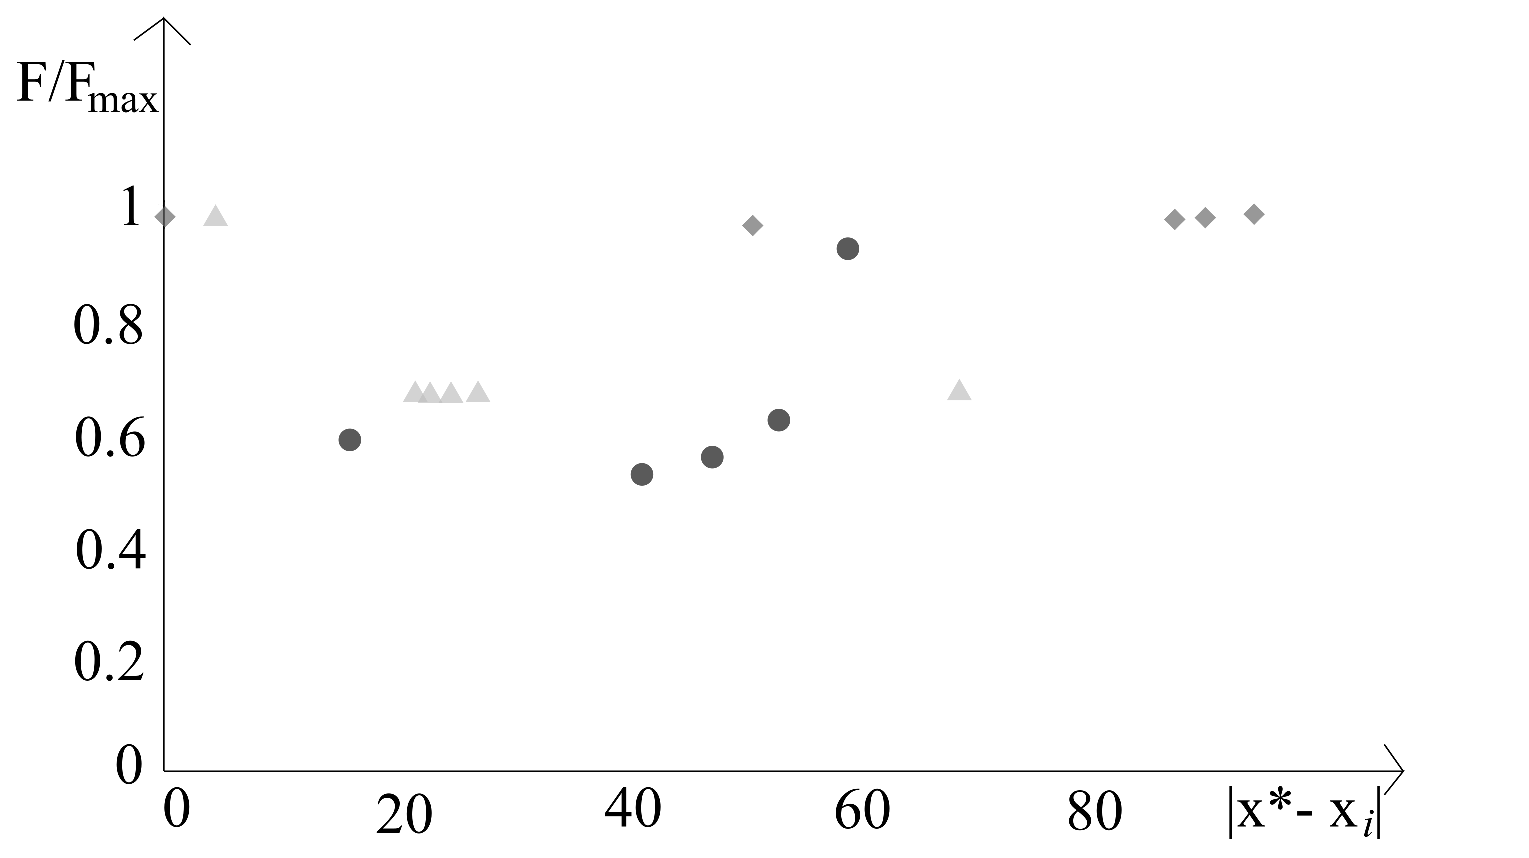
\includegraphics[width=0.9\linewidth]{fit_dist.eps} }
        \end{minipage}
        \vspace{0.7em}
        \caption{Зависимость качества локальных оптимумов от расстояния до глобального. Точками обозначены результаты для кольцевых решеток, состоящих из 8 излучателей, ромбами - для кольцевых решеток, состоящих из 16 излучателей, пятиугольниками - для СВД~3x3. }
        \label{ris:fit_dist1}
    \end{figure}
\end{frame}

\subsection{Область притяжения глобального оптимума}
\begin{frame}
    \frametitle{Область притяжения глобального оптимума}

    \begin{figure}
    \centering
        \begin{minipage}[h]{0.8\linewidth}
                \center{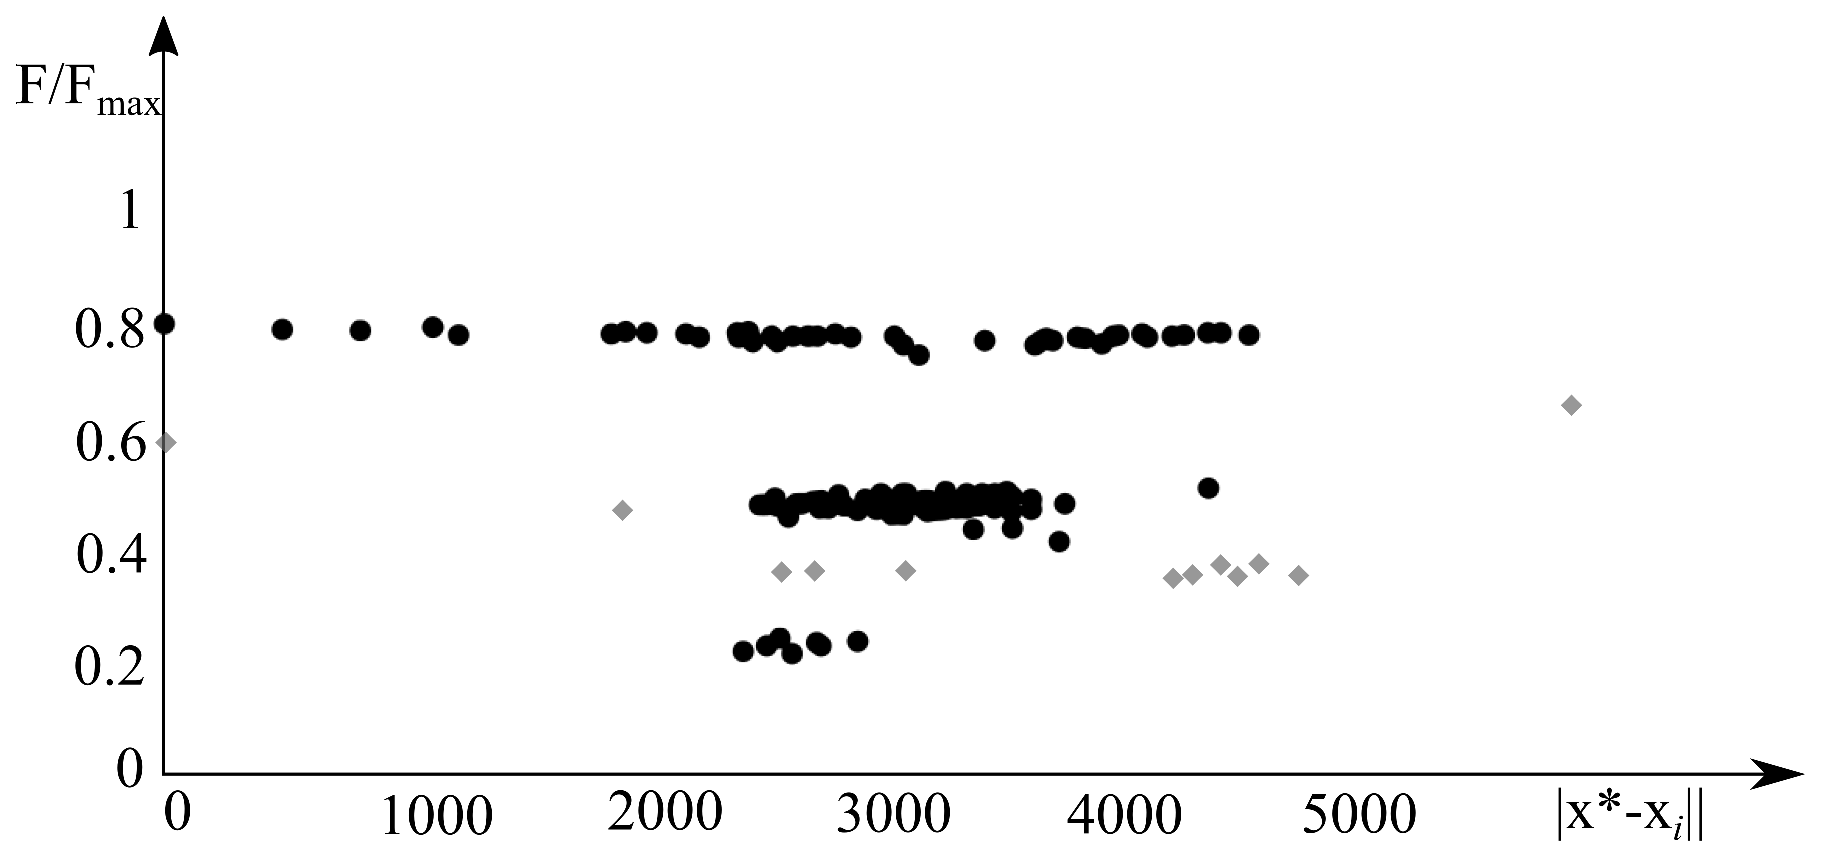
\includegraphics[width=0.9\linewidth]{fit_dist_2x2.eps} }
        \end{minipage}
        \vspace{0.7em}
        \caption{Зависимость качества локальных оптимумов от расстояния до глобального. Точками обозначены результаты для СВД'~2x2, ромбами - для СВД'~3x3.}
        \label{ris:fit_dist_2}
    \end{figure}

    Принимая на вход возмущенное порядка 0.5\% относительно нормы решение решателя BARON, градиентный подъем приводил к худшему решению.
\end{frame}

%------------------------------------------------

%\subsection{Дифференциальная эволюция}
%\begin{frame}
%    \frametitle{Дифференциальная эволюция}
%    // TODO: об алгоритма
%    \begin{itemize}
%      \item $v=v_{1}+f\cdot (v_{2}-v_{3}),$
%            где $v_1, v_2, v_3$ - случайные особи из текущей популяции, не равные друг другу.
%      \item Гибридный алгоритм с градиентным методом.
%    \end{itemize}
%\end{frame}

%------------------------------------------------
\section{Исследование возможностей ФАР в разных условиях}
\begin{frame}[plain, noframenumbering]
    \begin{center}
        \Huge
        Исследование возможностей ФАР в разных условиях
    \end{center}
\end{frame}

\begin{frame}
    \frametitle{Кольцевые ФАР}
    \begin{figure}
    \center{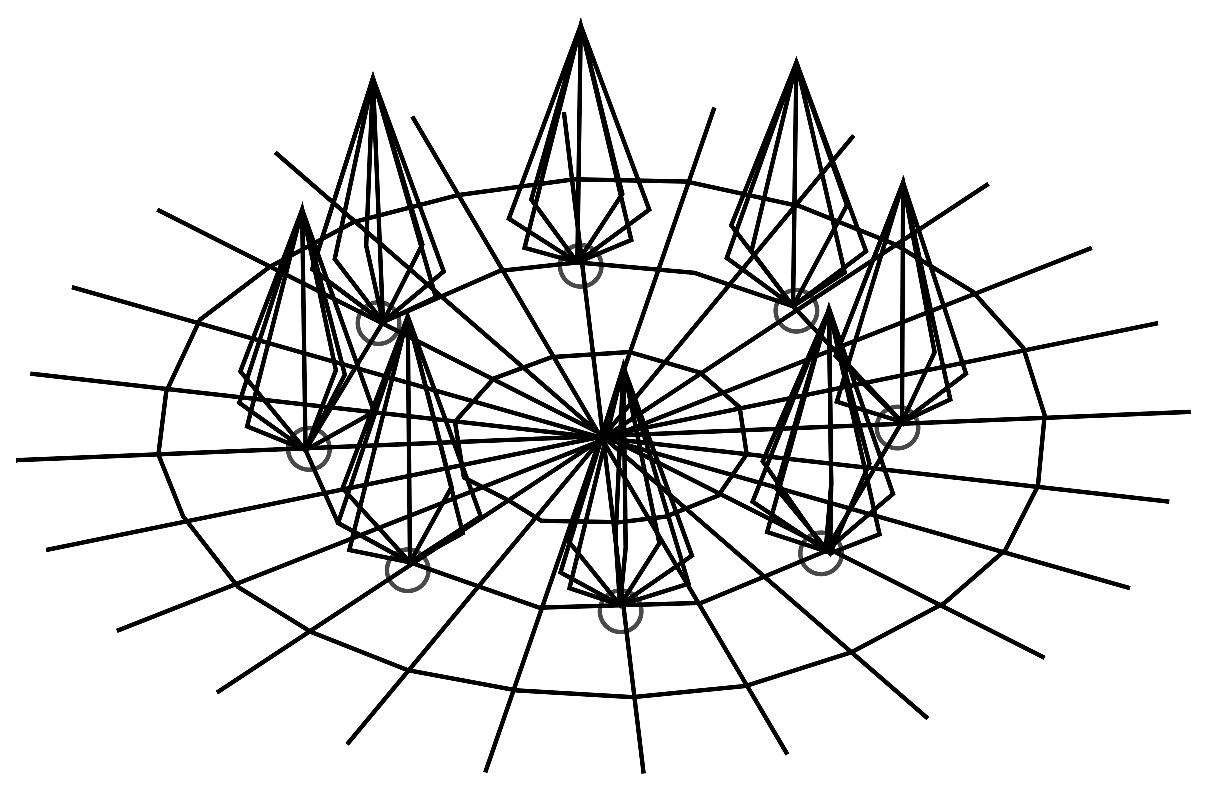
\includegraphics[width=0.6\linewidth]{r8.eps}}
    \caption{ФАР кольцевой структуры}
    \label{ris:rings}
    \end{figure}
\end{frame}

\subsection{Радиочастотные зависимости эффективности ФАР}
\begin{frame}
    \frametitle{Коэффициент усиления}

    \begin{figure}
    \center{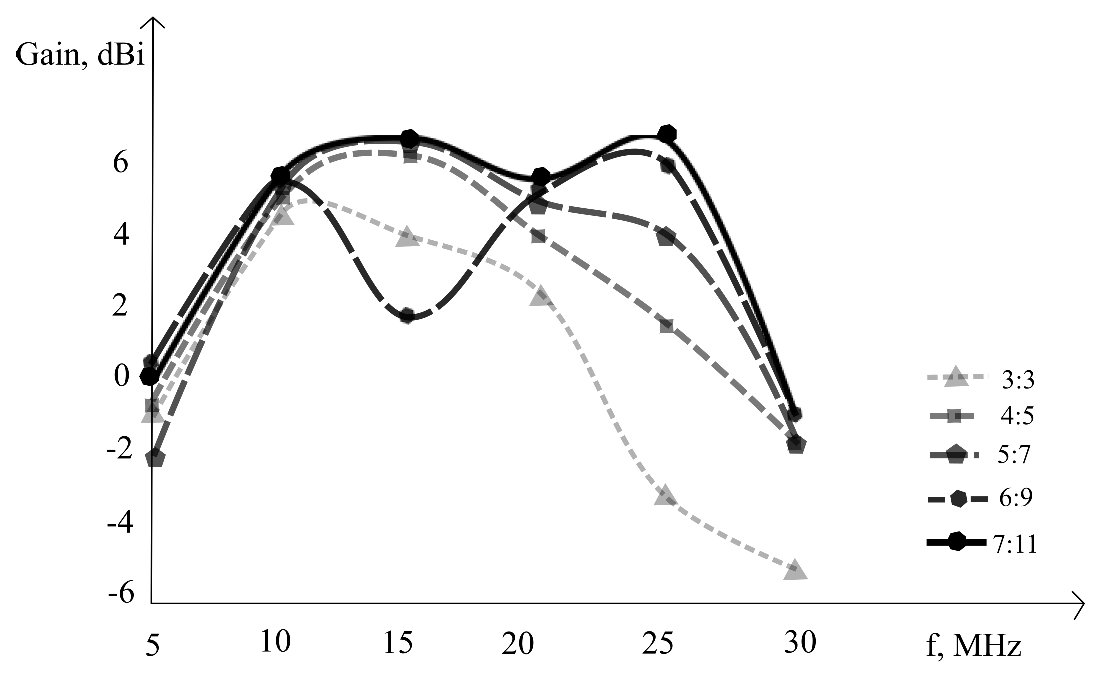
\includegraphics[width=0.8\linewidth]{ring_f__paa_gains.eps}}
    \caption{Зависимость коффициента усиления ФАР от частоты при птимизации в направлении 70:45}
    \label{ris:paa_gains_0}
    \end{figure}
\end{frame}

%------------------------------------------------

\begin{frame}
    \frametitle{Радиочастотные зависимости эффективности ФАР}
\begin{figure}
\center{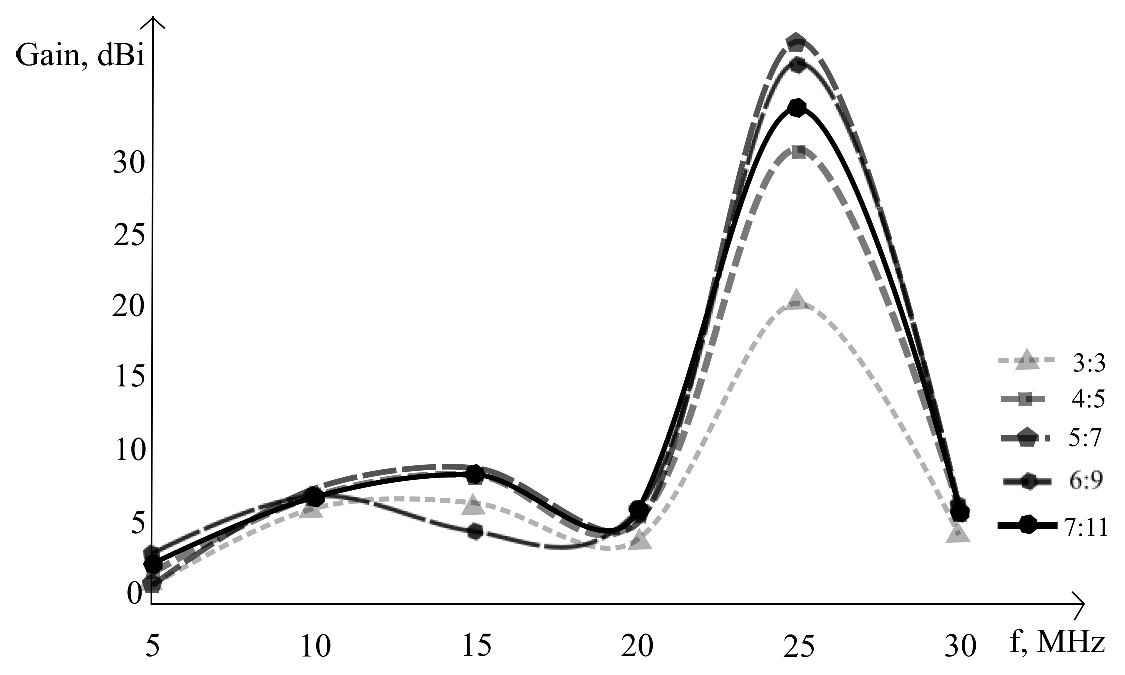
\includegraphics[width=0.5\linewidth]{ring_f_gains.eps}}
\label{ris:paa_gains}
\caption{Сравнение усиления ФАР и одиночного излучателя на различных частотах.}
\end{figure}

\begin{figure}
\begin{minipage}[h]{0.4\linewidth}
\center{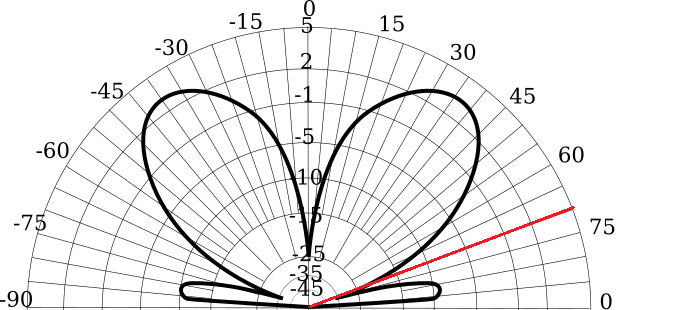
\includegraphics[width=1\linewidth]{r8_1_25_5x7_marked.png}} а)
\end{minipage}
\hfill
\begin{minipage}[h]{0.4\linewidth}
\center{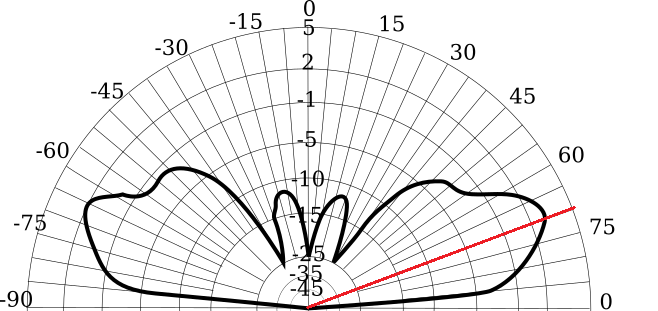
\includegraphics[width=1\linewidth]{r8_25_5x7_marked.png}} б)
\end{minipage}
\caption{Вертикальный план диаграммы направленности одиночного излучателя (a) и ФАР 5:7 (b) при 25МГц}
\label{ris:25MHz}
\end{figure}
\end{frame}


\subsection{Взаимное влияния излучателей}
\begin{frame}
    \frametitle{Взаимное влияния излучателей}
    \begin{figure}
    \begin{minipage}[h]{0.49\linewidth}
    \center{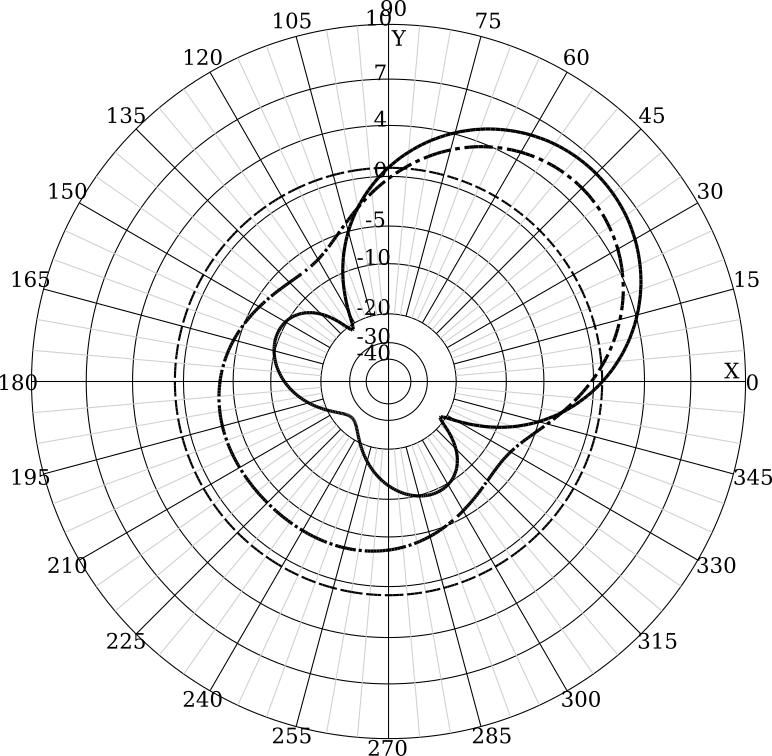
\includegraphics[width=1\linewidth]{r_bve_15_results_h.png} \\ а)}
    \end{minipage}
    \hfill
    \begin{minipage}[h]{0.49\linewidth}
    \center{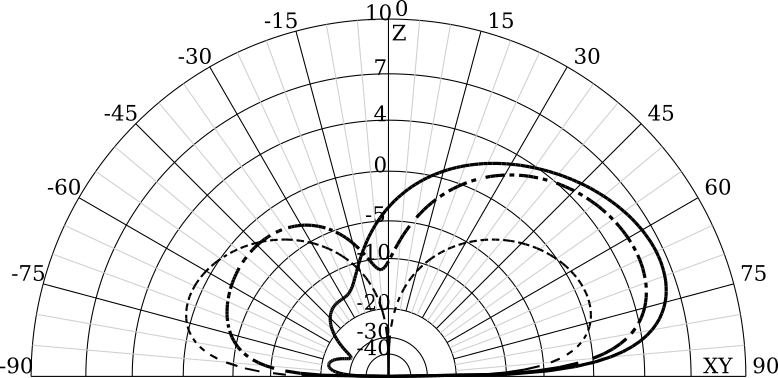
\includegraphics[width=1\linewidth]{r_bve_15_results_v.png} \\ б)}
    \end{minipage}
    \caption{Горизонтальный и вертикальный план диаграммы направленности ШВИ при расстоянии от центра излучателя до центра решетки 15 м. Пунктирной линией обозначено усиление одиночного излучателя, штрихпунктирной – простое фазирование, сплошной – решение задачи мат. программирования.}
    \label{pic:r_bve_15_results}
    \end{figure}
\end{frame}

\begin{frame}
    \frametitle{Взаимное влияния излучателей}
    \begin{figure}
    \begin{minipage}[h]{0.49\linewidth}
    \center{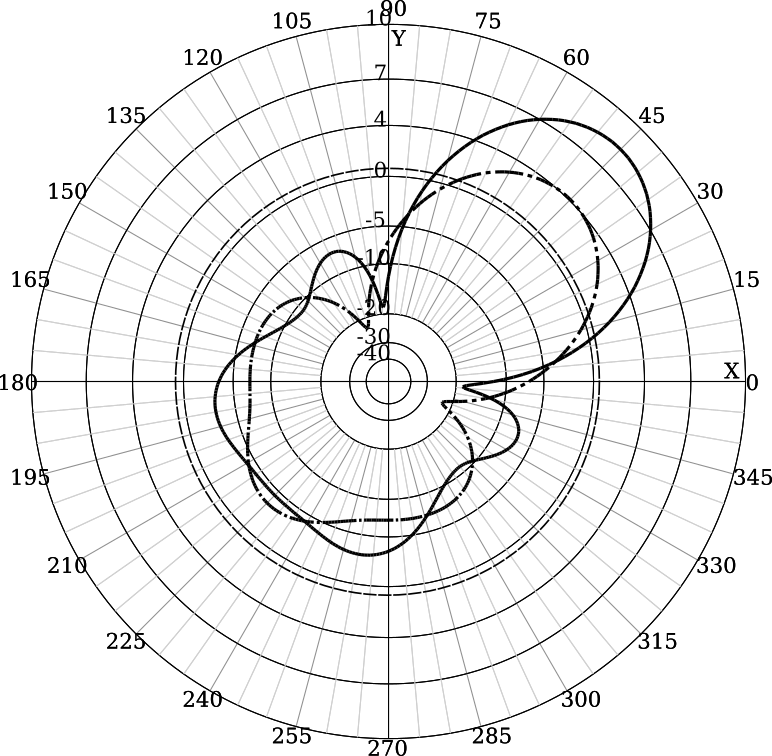
\includegraphics[width=1\linewidth]{r_bvd_20_results_h.png} \\ а)}
    \end{minipage}
    \hfill
    \begin{minipage}[h]{0.49\linewidth}
    \center{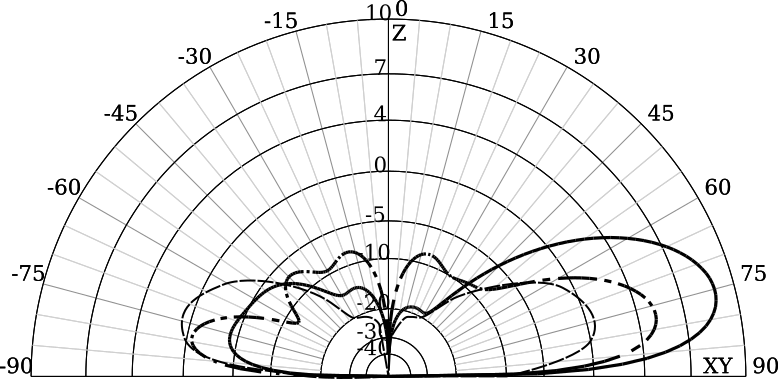
\includegraphics[width=1\linewidth]{r_bvd_20_results_v.png} \\ б)}
    \end{minipage}
    \caption{Горизонтальный (а) и вертикальный (б) план диаграммы направленности ШВД при расстоянии от центра излучателя до центра решетки 20 м. Пунктирной линией обозначено усиление одиночного излучателя, штрихпунктирной – простое фазирование, сплошной – решение задачи мат. программирования.}
    \label{pic:r_bvd_result_2}
    \end{figure}

\end{frame}

\begin{frame}
    \frametitle{Вывод}
    \begin{itemize}
      \item Показаны конфигурации ФАР, при которых учет взаимного влияния дает существенные преимущества перед простым фазированием.
    \end{itemize}
    \vspace{4em}

    \textbf{Tiunin N.:} On mutual influence of emitters in directivity optimization of shortwave phased antenna arrays~// Journal of Physics: Conference Series 2021,.
    
\vspace{1em}

    \textbf{Еремеев А.В., Тюнин Н.Н., Юрков А.С.:} Об оптимизации направленности коротковолновых фазированных антенных решеток кольцевой структуры~// Техника радиосвязи, 2022 (На рецензии).
\end{frame} 